\documentclass[12pt,a4paper]{memoir}
\usepackage[T1]{fontenc}
\usepackage[bahasai]{babel}
\usepackage{amsmath}
\usepackage{amsfonts}
\usepackage{amssymb}
\usepackage{makeidx}
\usepackage{graphicx}
\usepackage{verbatim}
\usepackage{tikz}
\usetikzlibrary{arrows.meta}
\usepackage[breakable]{tcolorbox}
\tcbset{nobeforeafter} % prevents tcolorboxes being placing in paragraphs
%\include{preamblejupyter}
\author{Novalio Daratha}
\title{Komputasi dengan Julia}
\begin{document}
	\maketitle
	\chapter{Bilangan Kompleks}
	
	Bahasa Julia memiliki tipe yang sudah didefinisikan untuk bilangan kompleks. Konstanta global $im$ dikaitkan dengan bilangan kompleks $i$, yang mewakili nilai akar kuadrat  dari $-1$, $\sqrt{-1}$. (Pemakaian simbol $i$ dan $j$ dilarang karena kedua simbol tersebut sering digunakan sebagai nama peubah indeks.) Gambar \ref{fig:complexnumber1} menunjukkan bagaimana memberikan nilai kompleks pada sebuah peubah bernama $S$.
	
	Bilangan kompleks bisa dikalikan dengan bilangan lainnya, ditambah, dikurangi, dikali atau dibagi. Hal ini juga ditunjukkan pada Gambar \ref{fig:complexnumber1}.

\begin{figure}[h]
	\centering
	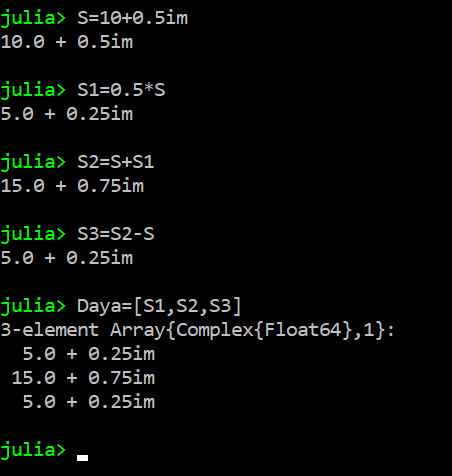
\includegraphics[width=0.7\linewidth]{images/complexnumber1}
	\caption{Memberikan nilai kompleks kepada sebuah peubah.}
	\label{fig:complexnumber1}
\end{figure}
	
	Sudut dan besar sebuah bilangan kompleks dapat dengan mudah menggunakan perintah \textbf{angle} dan \textbf{abs}. Gambar \ref{fig:complexnumber2} menunjukan hal-hal tersebut.
	
	\begin{figure}
		\centering
		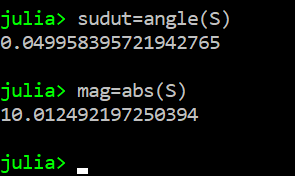
\includegraphics[width=0.7\linewidth]{images/complexnumber2}
		\caption{Sudut dan magnitude bilangan kompleks.}
		\label{fig:complexnumber2}
	\end{figure}
	
	Untuk mengubah bilangan kompleks dari bentuk polar ke rektangular juga cukup sederhana. Langkah pertama adalah menentukan nilai magnitude dan sudut (dalam radian). Kemudian bilangan kompleks diperoleh dengan menggunakan fungsi \textbf{Complex}. Contoh konversi ini dapat dilihat pada Gambar \ref{fig:complexnumber3}.
	
\begin{figure}
	\centering
	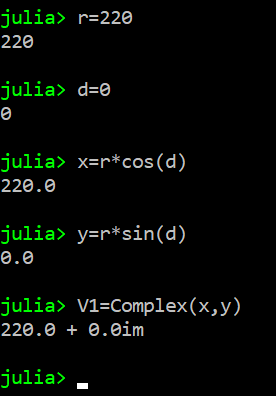
\includegraphics[width=0.35\linewidth]{images/complexnumber3}
	\caption{Mengubah bilangan kompleks dari bentuk polar ke rektangular.}
	\label{fig:complexnumber3}
\end{figure}

	Untuk mendapatkan conjugate sebuah bilangan complex, Anda dapat menggunakan fungsi \textbf{conj}. Fungsi \textbf{real} dan \textbf{imag} digunakan untuk mendapatkan nilai real dan imaginary sebuah bilangan kompleks. Anda bisa melihat contohnya di Gambar \ref{fig:complexnumber4}.
	
	\begin{figure}
		\centering
		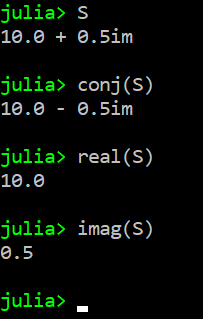
\includegraphics[width=0.4\linewidth]{images/complexnumber4}
		\caption{Contoh cara mendapatkan konjugate, bagian real dan bagian imajiner sebuah bilangan kompleks.}
		\label{fig:complexnumber4}
	\end{figure}
	\section{Sistem listrik tiga fasa}
	
	PLN menggunakan sistem tiga fasa untuk membangkitkan dan menyebarkan energi listrik. Secara matematis, tegangan listrik PLN dapat dimodelkan dengan vektor bilangan kompleks berikut ini.
	\begin{equation}
	\mathbf{V}
		\begin{bmatrix}
		\mathbf{V}_a\\
		\mathbf{V}_b\\
		\mathbf{V}_c
		\end{bmatrix}=
		\begin{bmatrix}
		220 \angle 0^o \\
		220 \angle -120^o \\
		220 \angle 220^o
		\end{bmatrix}=\begin{bmatrix}
		220\angle 0 \\
		220 \angle -2.0944\\
		220 \angle 2.0944
		\end{bmatrix}
	\end{equation}
Tegangan tiga fasa tersebut dapat dihitung dengan Julia seperti ditunjukkan pada Gambar \ref{fig:complexnumber5}.
\begin{figure}
	\centering
	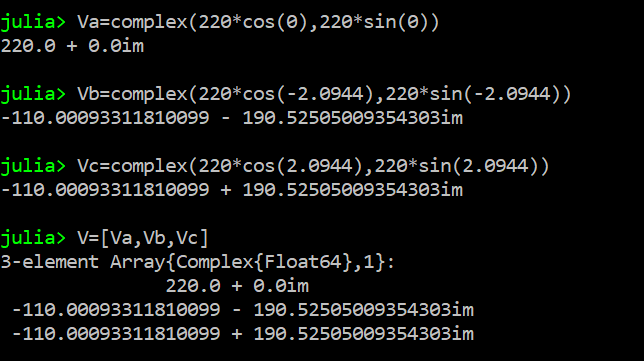
\includegraphics[width=0.7\linewidth]{images/complexnumber5}
	\caption{Tegangan tiga fasa yang disediakan PLN.}
	\label{fig:complexnumber5}
\end{figure}
	
	Untuk beban yang memerlukan daya sebesar

\begin{equation}
\mathbf{S}=
\begin{bmatrix}
\mathbf{S}_a\\
\mathbf{S}_b\\
\mathbf{S}_c
\end{bmatrix}=
\begin{bmatrix}
100 + 0j \\
200 + 100j \\
0 + 150j
\end{bmatrix},
\end{equation}

Daya tersebut dapat direpresentasikan dalam Julia seperti ditunjukkan dalam Gambar \ref{fig:complexnumber6}.

\begin{figure}
	\centering
	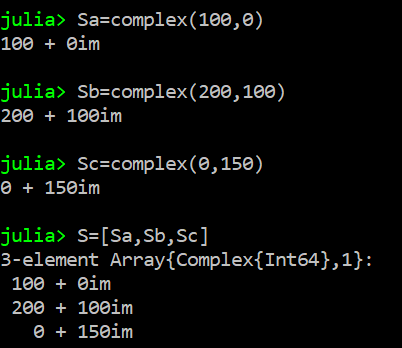
\includegraphics[width=0.7\linewidth]{images/complexnumber6}
	\caption{Cara merepresentasikan daya tiga fasa dalam Julia.}
	\label{fig:complexnumber6}
\end{figure}



PLN harus menyediakan arus sebesar konjugate dari hasil bagi daya dengan tegangan.

\begin{equation}
\mathbf{I}=(\mathbf{S/V})^*
\end{equation}

Perhitungan arus tersebut dapat dilakukan dengan proses pembagian per elemen yang menggunakan simbol "$./$". Simbol "/" tidak akan menghasilkan nilai yang kita maksud karena simbol "/" akan menghasilkan sebuah matriks $3 \times 3$ karena baik tegangan dan daya adalah matriks dengan ukuran $3 \times 1$. Hal ini ditunjukkan pada Gambar \ref{fig:complexnumber7}.

\begin{figure}
	\centering
	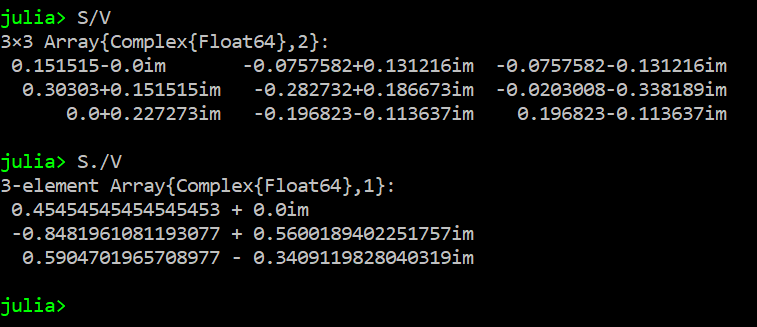
\includegraphics[width=1\linewidth]{images/complexnumber7}
	\caption{Cara menghitung arus beban apabila daya dan tegangan sudah diketahui. Perhatikan perbedaan simbol "/" dan "./" .}
	\label{fig:complexnumber7}
\end{figure}



\chapter{Komputasi iteratif (berulang)}
Dalam banyak situasi, kita perlu mengulang sederetan perhitungan berkali-kali. Komputer adalah alat yang sesuai untuk pekerjaan seperti itu. Dalam Bab ini, kita akan menggunakan struktur \textbf{for ... in ... end} untuk melakukan komputasi iteratif (berulang).

\section{Barisan dan Deret}
Barisan dan deret adalah contoh hal yang berulang.
\section{Barisan}
Marilah kita cetak 10 bilangan bulat positif pertama.
\begin{equation*}
B_1 =1,2,3,4,5,6,7,8,9,10.
\end{equation*}
Barisan $B_1$ tersebut dapat direpresentasikan dalam Julia dengan menggunakan perintah \textbf{range} seperti yang ditunjukan pada Gambar \ref{fig:barisan1}. 
\begin{figure}[h]
	\centering
	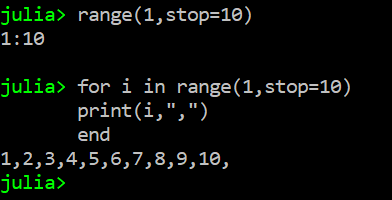
\includegraphics{images/barisan1}
	\caption{Barisan sepulu bilangan positif bulat pertama.}
	\label{fig:barisan1}
\end{figure}


Kemudian, marilah kita cetak sepuluh bilangan genap positif pertama.
\begin{equation*}
B_2 = 2,4,6,8,10,12,14,16,18,20.
\end{equation*}
Barisan $B_2$ juga dapat kita representasikan dengan perintah \textbf{range} seperti yang ditunjukkan pada Gambar.
\begin{figure}[h]
	\centering
	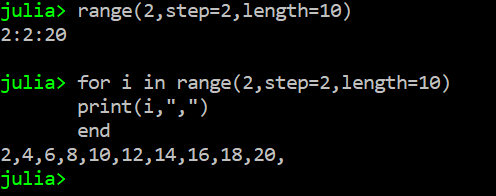
\includegraphics{images/barisan2}
	\caption{Barisan sepuluh bilangan genap positif pertama.}
	\label{fig:barisan2}
\end{figure}

Barisan $B_1$ dan $B_2$ adalah barisan yang sederhana. Bagaimana dengan barisan yang sedikit rumit yaitu barisan fibonaci berikut ini:
\begin{equation*}
B_3 =1,1,2,3,5,8,13,21,34,55.
\end{equation*}
Dalam hal ini, kita perlu mengingat kembali aturan dasar barisan fibonaci, yaitu

\begin{equation*}
fibonaci(n) =\begin{cases} 
1 & n=1 \\
1 & n=2 \\
f(n-1)+f(n-2) & n>2 
\end{cases}
\end{equation*}
Fungsi $fibonaci$ dapat dibuat dalam julia dengan menggunakan konsep \textbf{function ... end} dan \textbf{if ... elseif ... end} seperti ditunjukkan pada Gambar \ref{fig:barisanfibonaci}.

\begin{figure}[h]
	\centering
	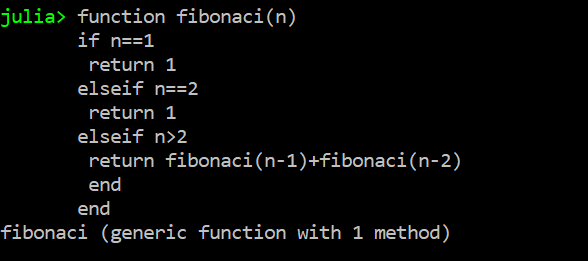
\includegraphics{images/barisanfibonaci}
	\caption{Fungsi fibonaci.}
	\label{fig:barisanfibonaci}
\end{figure}

Setelah fungsi fibonaci terdefinisi dalam Julia, kita bisa membuat barisan $B_3$ seperti yang ditunjukkan pada Gambar \ref{fig:barisanfibonaci2}.
\begin{figure}[h]
	\centering
	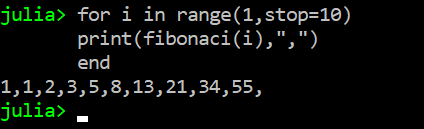
\includegraphics{images/barisanfibonaci2}
	\caption{Barisan fibonaci yang dihitung menggunakan fungsi yang didefinisikan sebelumnya di Gambar \ref{fig:barisanfibonaci}}
	\label{fig:barisanfibonaci2}
\end{figure}

\section{Deret}
Deret adalah jumlah dari elemen-elemen sebuah barisan. Misalnya, Jumlah sepuluh bilangan genap yang lebih besar dari 10 adalah
\begin{equation*}
D_1=\sum_{n=6}^{15} 2n=12+14+16+...+30.
\end{equation*}
Deret $D_1$ dapat dihitung dengan Julia seperti ditunjukkan pada Gambar \ref{fig:deret1}.

\begin{figure}
	\centering
	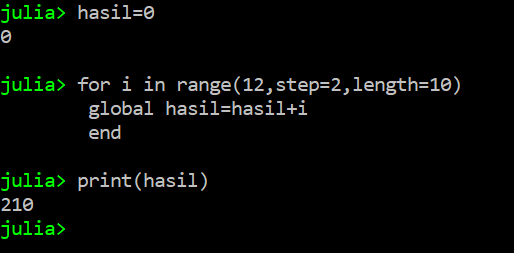
\includegraphics{images/deret1}
	\caption{Deret dapat dihitung dengan menggunakan Julia dan konsep perulangan dengan menggunakan \textbf{for ... in ... end}.}
	\label{fig:deret1}
\end{figure}
Kemudian, kita juga bisa menghitung deret fibonaci yang merupakan jumlah n bilangan fibonaci pertama.
\begin{equation*}
D_2[n]=1+1+2+3+5+8+...+fibonaci(n)
\end{equation*}
Deret $D_2$ dapat juga dihitung dengan Julia seperti ditunjukkan pada gambar 

\begin{figure}
	\centering
	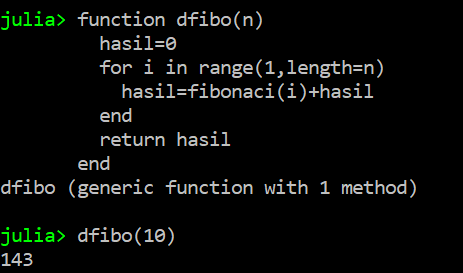
\includegraphics{images/deretfibo}
	\caption{Deret fibonaci.}
	\label{fig:deretfibo}
\end{figure}

\section{Aliran Daya Listrik}
Dalam analisis sistem tenaga listrik, ada kajian yang disebut kajian aliran daya. Di bagian ini, kita akan mencoba memecahkan soal aliran daya yang cukup sederhana. Perhatikan sebuah sistem sederhana yang ditunjukkan pada Gambar \ref{fig:stlsederhana}. Jika diketahui $V_0=220 + 0j  \;V, Z_{01}= 0.1 + 0.01j \Omega$ dan $S_1 = 100 + 50j \; \text{VA}$, carilah tegangan $V_1$.
\begin{figure}[h]
	\centering
\begin{tikzpicture}
\draw (0,0) -- (2,0) ;
\draw (3,0) -- (5,0) ;
\draw (2,0.2) -- node [above] {$Z_{01}$} (3,0.2);
\draw (2,-0.2) --(3,-0.2);
\draw (2, 0.2) -- (2, -0.2);
\draw (3,0.2) -- (3,-0.2) ;
\draw (0,-0.4) -- (0,+0.4) node[right]{$V_0$};
\draw (4.5,-0.4) -- (4.5,+0.4) node[right]{$V_1$};
\draw[-latex] (5,0)--(5,-0.5) node[right]{$S_1$};
\end{tikzpicture}
\caption{Sistem tenaga listrik sederhana}
\label{fig:stlsederhana}
\end{figure}

Untuk mencari besar $V_1$, langkah-langkah yang dapat dilakukan adalah:
\begin{enumerate}
	\item Mulai dengan $i=0$.
	\item Misalkan $V_1^0 = V_0$.
	\item Hitung arus dengan cara $I_1^0 =\left(\frac{S_1}{V_1}\right)^*$.
	\item mulai iterasi selanjutnya $i=i+1$
	\item Ganti nilai tegangan $V_1$  dengan nilai baru menggunakan $V_1^i =V_0 - I_1^{i-1}Z_{01}$
	\item Hitung arus dengan cara \[I_1^i =\left(\frac{S_1}{V_1^i}\right)^*\].
	\item Apakah syarat berikut terpenuhi?
	\[\left\lVert V_1^i - V_1^{i-1}) \right\rVert \leq \epsilon = 10^{-5}
	\]
	\begin{enumerate}
		\item Jika Ya, berhenti karena jawaban sudah diperoleh.
		\item Jika Tidak, ulangi langkah-langkah 4-7.  
	\end{enumerate}	 
\end{enumerate}

Langkah-langkah 1-7 adalah contoh algoritma yang memecahkan sebuah permasalah secara iteratif. Implementasi algoritma tersebut dalam Julia ditunjukkan pada Gambar \ref{fig:iterasi1}.
\begin{figure}
	\centering
	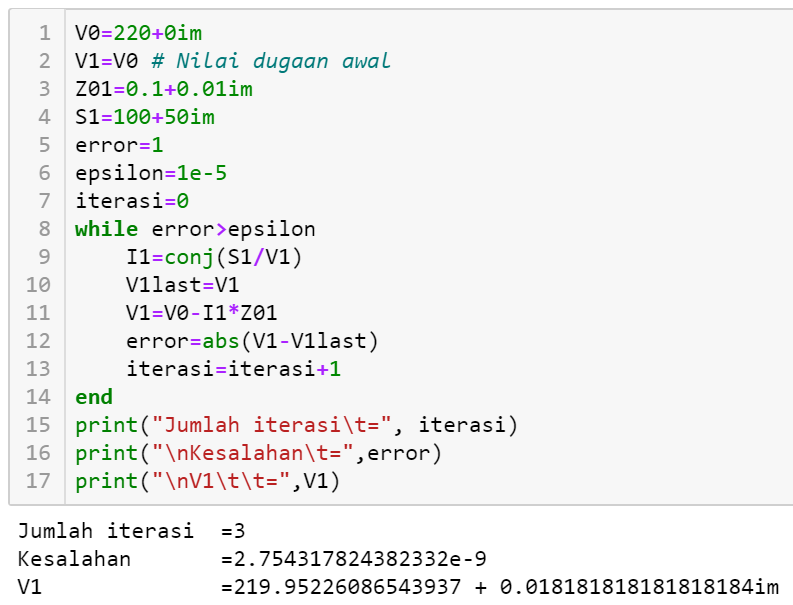
\includegraphics{images/iterasi1}
	\caption{Iterasi aliran daya listrik sederhana}
	\label{fig:iterasi1}
\end{figure}

\chapter{Algoritma Genetika}
Untuk memahami Bab ini, anda diharapkan sudah memahami algoritma genetika dengan cukup baik. Metode ini cukup mudah dipelajari dan banyak sumber di internet yang membahasnya.
\section{Permainan Kartu}
Ada sepuluh kartu yang diberi nomor 1 s/d 10. Kartu-kartu tersebut dibagi menjadi dua kelompok, A dan B. Kemudian, jumlah angka untuk masing-masing kelompok dihitung. Carilah cara pembagian yang meminimalkan selisih jumlah angka di kelompok A dan jumlah angka di kelompok B.
\subsection{Encoding}
Dalam pemanfaatan algoritma genetika, tahap encoding adalah tahap yang paling penting. Output dari tahap ini adalah struktur data yang cocok untuk masalah yang ingin dipecahkan dengan algoritma genetika.

Dalam hal ini sebuah gen adalah sebuah string yang memiliki 10 karakter karena kita memiliki 10 buah kartu. Setiap karakter dalam gen tersebut memiliki informasi yang berisi "A" ("B") jika kartu tersebut termasuk dalam kelompok "A" ("B"). Dalam gen tersebut, kartu ke-$i$ diwakili oleh karakter ke-$i$. Angka yang dimiliki oleh kartu ke-$i$ disimpan pada elemen ke-$i$ sebuah list bernama "w".

Sebagai contoh, untuk permainan kartu yang kita bahas di Sub bab ini, gen akan kita simpan dengan data berjenis \textbf{string}. Kemudian, setiap individu memiliki satu gen, satu sumA, satu sumB dan satu nilai fitness. Peubah sumA (sumB) adalah jumlah angka dari seluruh kartu yang ada di kelompok  A (B).
Nilai fitness didefinisikan sebagai berikut
\[
fitness=\left\lvert sumA-sumB \right\rvert,
\]
dimana, $\rvert\;\lvert$ menunjukkan nilai absolut. Kita mencari gen yang memiliki fitness sekecil mungkin atau sama dengan nol.

Encoding dapat dilakukan dalam Julia dengan memanfaatkan konsep \textbf{DataFrames}, \textbf{string} dan \textbf{rand} seperti ditunjukkan pada Gambar \ref{fig:ga1}.
\begin{figure}[h]
	\centering
	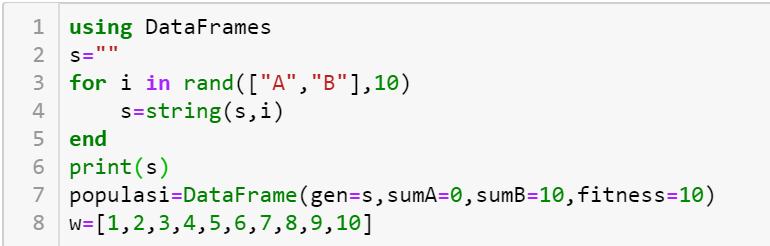
\includegraphics{images/ga1}
	\caption{Encoding permainan kartu untuk algoritma genetika. Sebuah gen adalah sebuah string yang memiliki 10 karakter karena kita memiliki 10 buah kartu. Setiap karakter dalam gen tersebut memiliki informasi yang berisi "A" ("B") jika kartu tersebut termasuk dalam kelompok "A" ("B"). Dalam gen tersebut, kartu ke-$i$ diwakili oleh karakter ke-$i$. Angka yang dimiliki oleh kartu ke-$i$ disimpan pada elemen ke-$i$ sebuah list bernama "w".}
	\label{fig:ga1}
\end{figure}

\subsection{Penghitungan nilai fitness}
Untuk setiap individu, berdasarkan gen yang dimilikinya, kita perlu menghitung fitnessnya. Oleh karena itu, kita perlu mendefinisikan fungsi yang sesuai kebutuhan tersebut dalam julia. Salah satu implementasinya ditunjukkan dalam Gambar \ref{fig:ga2}.
\begin{figure}[h]
	\centering
	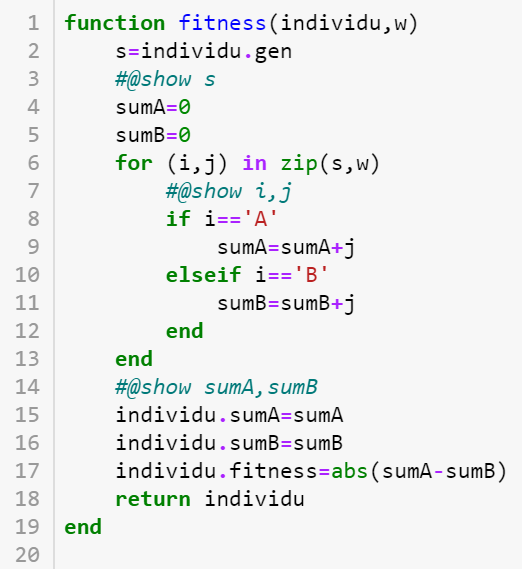
\includegraphics[width=0.7\linewidth]{images/ga2}
	\caption{Perhitungan nilai fitness sebuah gen.}
	\label{fig:ga2}
\end{figure}

\subsection{Gen dengan Nilai Acak}
Algoritma genetika memerlukan kemamputan untuk menghasilkan gen secara acak. Sesuai dengan encoding yang telah dipilih (lihat Gambar \ref{fig:ga1}). Kita dapat mendefinisikan sebuah fungsi yang menghasilkan gen secara acak seperti ditunjukkan pada Gambar \ref{fig:ga3}
\begin{figure}[h]
	\centering
	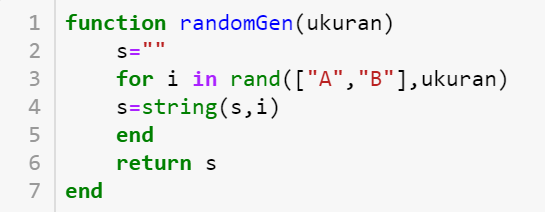
\includegraphics[width=0.7\linewidth]{images/ga3}
	\caption{Sebuah fungsi yang menghasilkan string secara acak yang terdiri dar abjad "A" atau "B" dengan jumlah huruf sesuai dengan nilai peubah "ukuran".}
	\label{fig:ga3}
\end{figure}

\subsection{Populasi Acak}
Algoritma Genetika juga membutuhkan fungsi untuk menghasilkan populasi dengan jumlah individu tertentu dengan gen acak. Hal ini dapat diimplementasikan dengan sebuah fungsi yang ditunjukkan pada Gambar \ref{fig:ga4}.

Fungsi untuk mencari populasi yang terdiri dari individu yang memiliki gen acak. Populasi disimpan dalam sebuah DataFrame. Jumlah individu dalam populasi sama dengan jumlah baris dalam dataframe yang dipakai. Kolom-kolom dalam DataFrame memuat informasi tentang gen,sumA, sumB dan fitness masing-masing individu.
\begin{figure}[h]
	\centering
	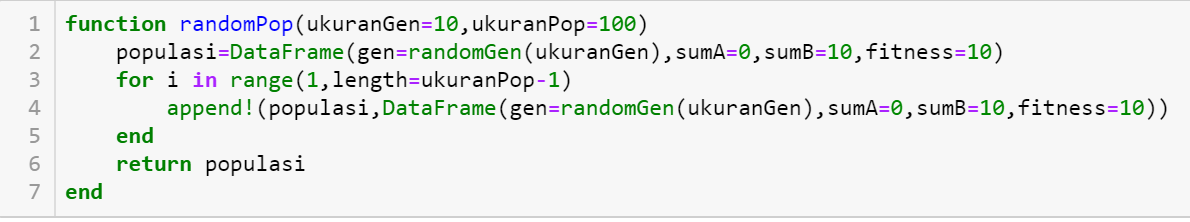
\includegraphics[width=\linewidth]{images/ga4}
	\caption{Fungsi untuk mencari populasi yang terdiri dari individu yang memiliki gen acak. Populasi disimpan dalam sebuah DataFrame. Jumlah individu dalam populasi sama dengan jumlah baris dalam dataframe yang dipakai. Kolom-kolom dalam DataFrame memuat informasi tentang gen,sumA, sumB dan fitness masing-masing individu.}
	\label{fig:ga4}
\end{figure}


\subsection{Evaluasi Populasi}
Algoritma Genetika juga membutuhkan fungsi evaluasi populasi. Dalam evaluasi ini ada dua hal utama yang dilakukan yaitu: penghitungan nilai fitness dan pengurutan berdasarkan nilai fitness.

\begin{figure}[h]
	\centering
	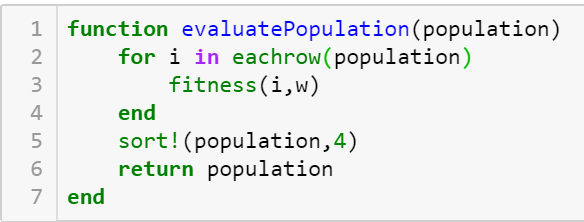
\includegraphics[width=0.7\linewidth]{images/ga5}
	\caption{Fungsi evaluasi populasi terdiri dari penghitungan nilai fitness sesuai dengan Gambar \ref{fig:ga2} dan pengurutan berdasarkan nilai fitness dengan menggunakan fungsi \textbf{sort!}. DataFrame populasi dijelaskan dalam Gambar \ref{fig:ga4}.}
	\label{fig:ga5}
\end{figure}

\subsection{Mutasi}
Mutasi adalah perubahan nilai gen. Hal ini juga bisa diimplementasikan dengan Julia seperti yang ditunjukkan dalam Gambar \ref{fig:ga6} yang menunjukan bagaimana merubah sebuah huruf dalam gen.

\begin{figure}[h]
	\centering
	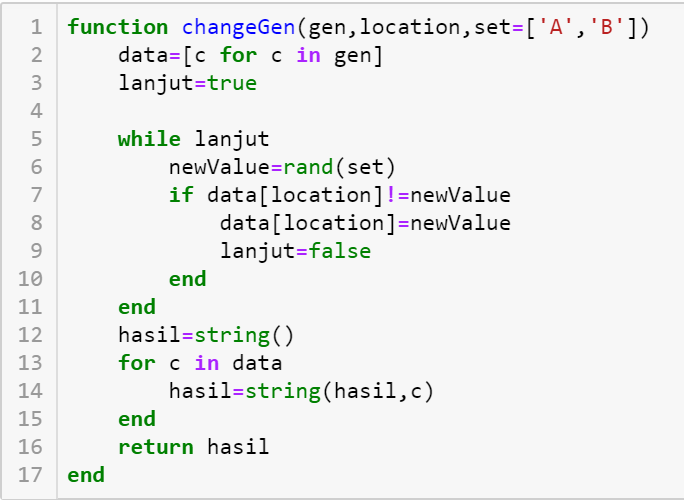
\includegraphics[width=0.7\linewidth]{images/ga6}
	\caption{Penggantian sebuah huruf dalam sebuah gen. Struktur \textbf{if .. then} memastikan bahwa penggantian hanya dilakukan apabila nilai baru berbeda dengan nilai yang ada. Struktur \textbf{while .. then} menjamin bahwa penggantian harus terjadi. }
	\label{fig:ga6}
\end{figure}

Kemudian, fungsi mutasi dalam sebuah populasi dapat dibuat. Input fungsi ini adalah populasi dan peluang terjadinya mutasi. Berdasarkan ukuran populasi dan peluang mutasi, individu yang  mengalami mutasi dipilih secara acak.


Input fungsi ini adalah populasi dan peluang terjadinya mutasi. Berdasarkan ukuran populasi dan peluang mutasi, individu yang  mengalami mutasi dipilih secara acak. Lokasi terjadinya mutasi pun dipilih secara acak. Output fungsi ini adalah populasi baru yang sebagian kecil individunya telah mengalami mutasi.
\begin{figure}
	\centering
	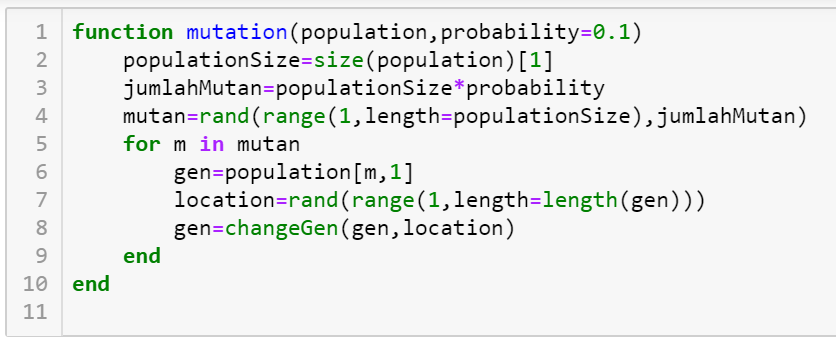
\includegraphics[width=\linewidth]{images/ga7}
	\caption{Fungsi mutasi dalam sebuah populasi. Input fungsi ini adalah populasi dan peluang terjadinya mutasi. Berdasarkan ukuran populasi dan peluang mutasi, individu yang  mengalami mutasi dipilih secara acak. Lokasi terjadinya mutasi pun dipilih secara acak. Output fungsi ini adalah populasi baru yang sebagian kecil individunya telah mengalami mutasi.}
	\label{fig:ga7}
\end{figure}


\end{document}